% Options for packages loaded elsewhere
\PassOptionsToPackage{unicode}{hyperref}
\PassOptionsToPackage{hyphens}{url}
%
\documentclass[
  12pt,
]{article}
\usepackage{amsmath,amssymb}
\usepackage{lmodern}
\usepackage{iftex}
\ifPDFTeX
  \usepackage[T1]{fontenc}
  \usepackage[utf8]{inputenc}
  \usepackage{textcomp} % provide euro and other symbols
\else % if luatex or xetex
  \usepackage{unicode-math}
  \defaultfontfeatures{Scale=MatchLowercase}
  \defaultfontfeatures[\rmfamily]{Ligatures=TeX,Scale=1}
  \setmainfont[]{Times New Roman}
\fi
% Use upquote if available, for straight quotes in verbatim environments
\IfFileExists{upquote.sty}{\usepackage{upquote}}{}
\IfFileExists{microtype.sty}{% use microtype if available
  \usepackage[]{microtype}
  \UseMicrotypeSet[protrusion]{basicmath} % disable protrusion for tt fonts
}{}
\makeatletter
\@ifundefined{KOMAClassName}{% if non-KOMA class
  \IfFileExists{parskip.sty}{%
    \usepackage{parskip}
  }{% else
    \setlength{\parindent}{0pt}
    \setlength{\parskip}{6pt plus 2pt minus 1pt}}
}{% if KOMA class
  \KOMAoptions{parskip=half}}
\makeatother
\usepackage{xcolor}
\usepackage[margin=2.54cm]{geometry}
\usepackage{longtable,booktabs,array}
\usepackage{calc} % for calculating minipage widths
% Correct order of tables after \paragraph or \subparagraph
\usepackage{etoolbox}
\makeatletter
\patchcmd\longtable{\par}{\if@noskipsec\mbox{}\fi\par}{}{}
\makeatother
% Allow footnotes in longtable head/foot
\IfFileExists{footnotehyper.sty}{\usepackage{footnotehyper}}{\usepackage{footnote}}
\makesavenoteenv{longtable}
\usepackage{graphicx}
\makeatletter
\def\maxwidth{\ifdim\Gin@nat@width>\linewidth\linewidth\else\Gin@nat@width\fi}
\def\maxheight{\ifdim\Gin@nat@height>\textheight\textheight\else\Gin@nat@height\fi}
\makeatother
% Scale images if necessary, so that they will not overflow the page
% margins by default, and it is still possible to overwrite the defaults
% using explicit options in \includegraphics[width, height, ...]{}
\setkeys{Gin}{width=\maxwidth,height=\maxheight,keepaspectratio}
% Set default figure placement to htbp
\makeatletter
\def\fps@figure{htbp}
\makeatother
\setlength{\emergencystretch}{3em} % prevent overfull lines
\providecommand{\tightlist}{%
  \setlength{\itemsep}{0pt}\setlength{\parskip}{0pt}}
\setcounter{secnumdepth}{5}
\ifLuaTeX
  \usepackage{selnolig}  % disable illegal ligatures
\fi
\IfFileExists{bookmark.sty}{\usepackage{bookmark}}{\usepackage{hyperref}}
\IfFileExists{xurl.sty}{\usepackage{xurl}}{} % add URL line breaks if available
\urlstyle{same} % disable monospaced font for URLs
\hypersetup{
  pdftitle={Analyzing Soil Moisture \& Precipitation Trends in Coweeta Basin LTER Site},
  pdfauthor={Kelly Davidson, Megan McClaugherty, \& Isabel Zungailia},
  hidelinks,
  pdfcreator={LaTeX via pandoc}}

\title{Analyzing Soil Moisture \& Precipitation Trends in Coweeta Basin
LTER Site}
\usepackage{etoolbox}
\makeatletter
\providecommand{\subtitle}[1]{% add subtitle to \maketitle
  \apptocmd{\@title}{\par {\large #1 \par}}{}{}
}
\makeatother
\subtitle{Web address for GitHub repository}
\author{Kelly Davidson, Megan McClaugherty, \& Isabel Zungailia}
\date{}

\begin{document}
\maketitle

\newpage
\tableofcontents 
\newpage
\listoftables 
\newpage
\listoffigures 
\newpage

\hypertarget{rationale-and-research-questions}{%
\section{Rationale and Research
Questions}\label{rationale-and-research-questions}}

\begin{figure}
\centering
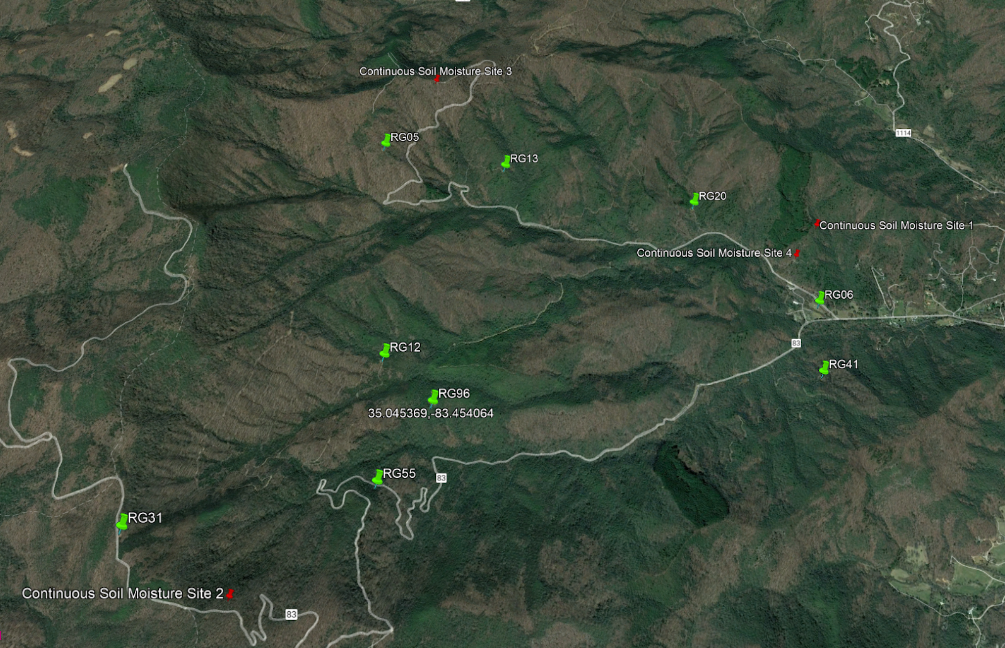
\includegraphics{"/home/guest/Zungailia_Davidson_McClaugherty/Data/precipandsmois.png"}
\caption{Study Sites and Recording Rain Gage Locations}
\end{figure}

\newpage

\hypertarget{dataset-information}{%
\section{Dataset Information}\label{dataset-information}}

\textbf{Data Description} Soil moisture datasets were collected from the
EDI Data Portal for Coweeta LTER
\href{https://portal.edirepository.org/nis/home.jsp}{this is a link.}.
Coweeta LTER (248) was selected as the LTER Site and ``Continuously
measured forest soil moisture at four sites in the Coweeta Basin'''' was
selected as the dataset of interest. The data were accessed 11/21/22.
The following selections were downloaded:\\
1. 1040\_2000\_2014\\
2. 1040.kml (a Google Earth file showing the soil moisture site
locations)\\
Precipitation data was collected from the US Forest Service Southern
Research Station
\href{https://www.srs.fs.usda.gov/coweeta/tools-and-data/}{this is a
link.}. Daily precipitation data from recording rain gages (RRG) at
Coweeta Hydrologic Lab, North Carolina was selected under Coweeta
Datasets on the USFS Research Data Archive
\href{https://www.fs.usda.gov/rds/archive/Catalog/RDS-2017-0031}{this is
a link.}. Data were accessed 11/30/22.

We generated four new datasets combining the monthly average
precipitation with monthly average 30 cm soil moisture at the 4 sites
monitored at the Coweeta LTER.

\textbf{Data Wrangling} The initial datasets required a significant
amount of wrangling before they could be used for analysis. The raw soil
moisture data had 21 variables/columns, so the first step was to select
the columns of interest (site, Year, YearDay, smois30). A new `Date'
column was created (format = ``\%Y-\%j'') and the data was filtered to
exclude the smois30 values less than 0 and greater than 1 (since soil
moisture is expressed as percent water content). All NAs were omitted
from the data and it was then split into 4 separate dataframes (one per
site). The smois30 (cm) values were averaged per month for each site
prior to analysis.

The raw precipitation datasets (for the three rain gauges) had 5
variables (YEAR, MONTH, DAY, RRG''gauge ID number''). A new `Date'
column was created (format = ``\%Y-\%m-\%d''), and the data was wrangled
to only include the same years that are represented by the soil moisture
data (2000-2013). All NAs were omitted from the data. The final step was
to average the rain gauge data by month (to align with the soil moisture
monthly averages).

\textbf{Data Structure} Processed Soil Moisture Data

\begin{longtable}[]{@{}
  >{\raggedleft\arraybackslash}p{(\columnwidth - 8\tabcolsep) * \real{0.2143}}
  >{\centering\arraybackslash}p{(\columnwidth - 8\tabcolsep) * \real{0.2857}}
  >{\raggedleft\arraybackslash}p{(\columnwidth - 8\tabcolsep) * \real{0.1667}}
  >{\centering\arraybackslash}p{(\columnwidth - 8\tabcolsep) * \real{0.1667}}
  >{\centering\arraybackslash}p{(\columnwidth - 8\tabcolsep) * \real{0.1667}}@{}}
\toprule()
\begin{minipage}[b]{\linewidth}\raggedleft
Variable
\end{minipage} & \begin{minipage}[b]{\linewidth}\centering
Description
\end{minipage} & \begin{minipage}[b]{\linewidth}\raggedleft
Units
\end{minipage} & \begin{minipage}[b]{\linewidth}\centering
Class
\end{minipage} & \begin{minipage}[b]{\linewidth}\centering
Stats
\end{minipage} \\
\midrule()
\endhead
Year & Calendar year & & Integer & Minimum = 2000, Maximum = 2013 \\
Month & Calendar Month & & Integer & Minimum = 01 (January), Maximum =
07 (July) \\
AverageMonthlySmois30 & Unitless (measured as a percent) & Numeric &
Site 1: minimum = 0.1521, mean = 0.2804, maximum = 0.3556, Site 2:
minimum = 0.1046, mean = 0.2543, maximum = 0.3421, Site 3: minimum =
0.114, mean = 0.2729, maximum = 0.5753, Site 4: minimum = 0.1383, mean =
0.3156, maximum = 0.4922 & \\
YearMonth & Date in format YYYY-MM-DD & & Character & Minimum =
2000-01-21, Maximum = 2013-07-19 \\
\bottomrule()
\end{longtable}

Processed Rain Gauge/Precipitation Data Variable \textbar{} Description
\textbar{} Units \textbar{} Class \textbar{} Stats

\newpage

\hypertarget{exploratory-analysis}{%
\section{Exploratory Analysis}\label{exploratory-analysis}}

\newpage

\hypertarget{analysis}{%
\section{Analysis}\label{analysis}}

\hypertarget{question-1-insert-specific-question-here-and-add-additional-subsections-for-additional-questions-below-if-needed}{%
\subsection{Question 1: \textless insert specific question here and add
additional subsections for additional questions below, if
needed\textgreater{}}\label{question-1-insert-specific-question-here-and-add-additional-subsections-for-additional-questions-below-if-needed}}

\hypertarget{question-2}{%
\subsection{Question 2:}\label{question-2}}

\newpage

\hypertarget{summary-and-conclusions}{%
\section{Summary and Conclusions}\label{summary-and-conclusions}}

\newpage

\hypertarget{references}{%
\section{References}\label{references}}

\textless add references here if relevant, otherwise delete this
section\textgreater{}

\end{document}
